\documentclass[tikz,border=7pt]{standalone}
\usepackage{amsmath,amssymb}
\usetikzlibrary{arrows.meta,calc,positioning}

\definecolor{ink}{HTML}{243447}
\definecolor{muted}{HTML}{64748B}
\definecolor{safe}{HTML}{2563A6}
\definecolor{safeLight}{HTML}{BFDBFE}
\definecolor{danger}{HTML}{C43D3D}
\definecolor{dangerLight}{HTML}{FAD4D4}
\definecolor{panelFill}{HTML}{F8FAFC}

\tikzset{
    >={Latex[length=2.2mm,width=1.6mm]},
    panel/.style={draw=ink!25, fill=panelFill, rounded corners=3pt, line width=0.7pt},
    safe path/.style={safe, line width=1.7pt, -{Latex[length=2.4mm]}},
    learned path/.style={danger, line width=2pt, -{Latex[length=2.5mm]}},
    velocity/.style={safe, line width=1.25pt, -{Latex[length=2mm]}},
    average/.style={danger, line width=1.6pt, -{Latex[length=2.2mm]}},
    root node/.style={circle, draw=ink, fill=white, line width=0.9pt,
                     minimum size=7mm, inner sep=0pt,
                     font=\sffamily\scriptsize},
    lineage node/.style={circle, draw=safe, fill=safeLight!55,
                        line width=0.9pt, minimum size=7mm, inner sep=0pt,
                        font=\sffamily\scriptsize},
    invalid node/.style={circle, draw=danger, fill=dangerLight,
                        line width=1pt, minimum size=7mm, inner sep=0pt,
                        font=\sffamily\bfseries\scriptsize, text=danger},
    failure note/.style={rounded corners=2.5pt, draw=danger!55,
                        fill=dangerLight!35, line width=0.7pt,
                        minimum width=55mm, minimum height=10mm,
                        inner sep=4pt, align=left,
                        font=\sffamily\scriptsize, text=ink},
    badge/.style={circle, fill=danger, text=white, draw=white,
                 line width=0.7pt, minimum size=5.5mm, inner sep=0pt,
                 font=\sffamily\bfseries\tiny},
    label text/.style={font=\sffamily\scriptsize, text=ink},
    small note/.style={font=\sffamily\tiny, text=muted, align=center},
    title/.style={font=\sffamily\bfseries\small, text=ink},
}

\begin{document}
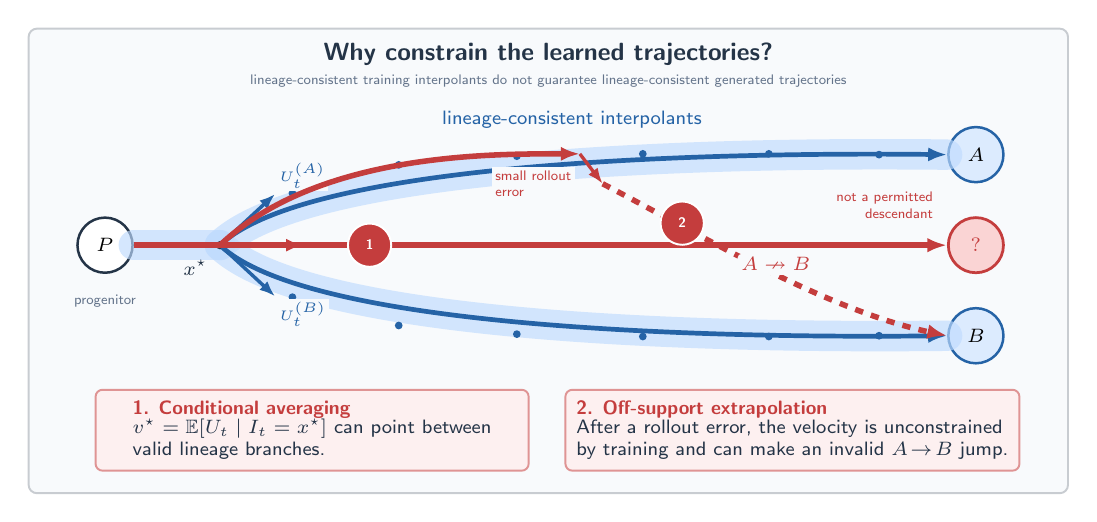
\begin{tikzpicture}[font=\sffamily]

% One lineage tree, with valid interpolants and two distinct failure modes.
\draw[panel] (-0.25,-3.15) rectangle (12.95,2.75);
\node[title] at (6.35,2.42) {Why constrain the learned trajectories?};
\node[small note] at (6.35,2.08)
    {lineage-consistent training interpolants do not guarantee lineage-consistent generated trajectories};

% Valid lineage tree and the support of the training interpolants.
\node[root node] (P) at (0.72,0) {$P$};
\node[small note, below=4pt] at (P.south) {progenitor};
\coordinate (branch) at (2.18,0);
\node[lineage node] (A) at (11.78,1.15) {$A$};
\node[lineage node] (B) at (11.78,-1.15) {$B$};
\node[invalid node] (Q) at (11.78,0) {$?$};

\draw[safeLight, line width=11pt, line cap=round, opacity=0.65]
    (P.east) -- (branch);
\draw[safeLight, line width=11pt, line cap=round, opacity=0.65]
    (branch) .. controls (3.42,1.18) and (9.55,1.17) .. (A.west);
\draw[safeLight, line width=11pt, line cap=round, opacity=0.65]
    (branch) .. controls (3.42,-1.18) and (9.55,-1.17) .. (B.west);
\draw[safe, line width=1.7pt] (P.east) -- (branch);
\draw[safe path]
    (branch) .. controls (3.42,1.18) and (9.55,1.17) .. (A.west);
\draw[safe path]
    (branch) .. controls (3.42,-1.18) and (9.55,-1.17) .. (B.west);
\node[label text, text=safe] at (6.65,1.60)
    {lineage-consistent interpolants};

\foreach \x/\y in {3.10/0.66,4.45/1.02,5.95/1.13,7.55/1.16,9.15/1.16,10.55/1.15,
                     3.10/-0.66,4.45/-1.02,5.95/-1.13,7.55/-1.16,9.15/-1.16,10.55/-1.15} {
    \fill[safe] (\x,\y) circle (1.4pt);
}

% Failure 1: the conditional mean points between the two admissible branches.
\fill[ink] (branch) circle (1.5pt);
\node[label text, below left=2pt and 1pt] at (branch) {$x^\star$};
\draw[velocity] (branch) -- (2.88,0.65);
\draw[velocity] (branch) -- (2.88,-0.65);
\node[small note, text=safe, fill=panelFill, inner sep=1pt, anchor=west]
    at (2.90,0.88) {$U_t^{(A)}$};
\node[small note, text=safe, fill=panelFill, inner sep=1pt, anchor=west]
    at (2.90,-0.88) {$U_t^{(B)}$};
\draw[learned path] (P.east) -- (branch) -- (Q.west);
\draw[average] (branch) -- (3.24,0);
\node[badge] at (4.08,0) {1};
\node[small note, text=danger, align=right, anchor=south east]
    at (11.36,0.22) {not a permitted\\descendant};

% Failure 2: a rollout leaves the supervised branches and jumps lineages.
\draw[danger, line width=2pt, -{Latex[length=2.4mm]}]
    (branch) .. controls (3.42,1.18) and (5.65,1.16) .. (6.75,1.16);
\draw[danger, line width=1.2pt, -{Latex[length=2mm]}]
    (6.75,1.16) -- (7.04,0.78);
\node[small note, text=danger, fill=panelFill, inner sep=1.2pt,
      align=left, anchor=east]
    at (6.69,0.78) {small rollout\\error};
\draw[danger, dashed, line width=2pt, -{Latex[length=2.5mm]}]
    (7.04,0.78) .. controls (8.16,0.20) and (9.85,-0.82) .. (B.west);
\node[badge] at (8.05,0.28) {2};
\node[font=\sffamily\bfseries\scriptsize, text=danger,
      fill=panelFill, rounded corners=2pt, inner sep=1.5pt]
    at (9.24,-0.24) {$A\nrightarrow B$};

% Compact explanations keyed to the two red trajectories above.
\node[failure note] at (3.35,-2.35)
    {\textcolor{danger}{\bfseries 1. Conditional averaging}\\[-1pt]
     $v^\star=\mathbb E[U_t\mid I_t=x^\star]$ can point between\\
     valid lineage branches.};
\node[failure note] at (9.45,-2.35)
    {\textcolor{danger}{\bfseries 2. Off-support extrapolation}\\[-1pt]
     After a rollout error, the velocity is unconstrained\\
     by training and can make an invalid $A\!\to\!B$ jump.};

\end{tikzpicture}
\end{document}
